\chapter{Introduction to Distributed System}
\subsection{Distributed System Definition}
The definition of Distributed System can be given in two ways:
\begin{itemize}
    \item A \textbf{distributed system} is a system in which components located as \textit{networking computers} communicate and coordinate their actions only by passing messages. It is a set of \textbf{autonomous nodes} that interact and collaborate in order to reach a particular goal. Computers that are connected by a network may be spatially separated by any distance, and they communicate by exchanging information through a communication network.
    \item A \textbf{distributed system} is composed of \textit{more than one autonomous computer system} that interacts to \textbf{reach a given goal}. Nodes are autonomous since they can work alone, maintaining processes and data. The distributed systems are different from parallel systems, in which the main focus is the execution of a single application using several cores.
\end{itemize}

\subsection{Cloud Computing Definition}
Moreover we can define also \textbf{Cloud Computing,} it is a specialized form of distributed computing that introduces \textit{utilization models} for remotely provisioning scalable and \textit{measured resources}. Further we can define its five essential characteristics, its three service models ad its four deployment models.
\begin{itemize}
    \item \textbf{Characteristics:}
    \begin{itemize}
        \item On-demand self service
        \item Measured service
        \item Broad network access
        \item Rapid elasticity
        \item Resource pooling
    \end{itemize}
    \item \textbf{Service models:}
    \begin{itemize}
        \item Software as a service
        \item Platform as a service
        \item Infrastructure as a service
    \end{itemize}
    \item \textbf{Deployment modules:}
    \begin{itemize}
        \item Public Clouds
        \item Private Clouds
        \item Hybrid Clouds
        \item Community Clouds
    \end{itemize}
\end{itemize}

\section{Advantages}
Distributed System has lots of advantages:
\begin{itemize}
    \item \textbf{Resource sharing:} sharing of hardware and software resources
    \item \textbf{Heterogeneity:} it can be composed of different components
    \item \textbf{Reliability:} if there is a crash the system is still alive
    \item \textbf{Extendibility / Scalability}:
        \begin{itemize}
            \item \textit{Extendibility:} possibility to include another node in the system
            \item \textit{Scalability:} possibility of including a new node of the same type
        \end{itemize}
    \item \textbf{Performance:} they offer results in an efficient way and optimum values of throughput and response time.
    \item \textbf{Transparency:} is defined as \textit{hiding} the separation of components in a distribution system from the user and the application program. In a way such that the system is \textit{perceived as a whole} rather than as a \textit{collection of independent components}.
\end{itemize}

\section{Features}
Distributed System has lots of features:
\begin{itemize}
    \item \textbf{Concurrency:} nodes can work in parallel
    \item \textbf{Autonomous and asynchronous:} a node can survive alone and each machine has its own clock
    \item \textbf{Resource sharing:} access to resources can be shared, so a DS implements a strategy to manage them
    \item \textbf{Lack of global time:} when a process need to cooperate they coordinate their actions by exchanging messages. Since each machine is composed of its own clock, they are not able to coordinate synchronously.
    \item \textbf{Faults independent:} all computer system can fail, and it is their responsibility to design a plan for the consequences of possible failures. Possible faults of nodes do not affect other nodes in the network.
\end{itemize}
\begin{figure}
    \centering
    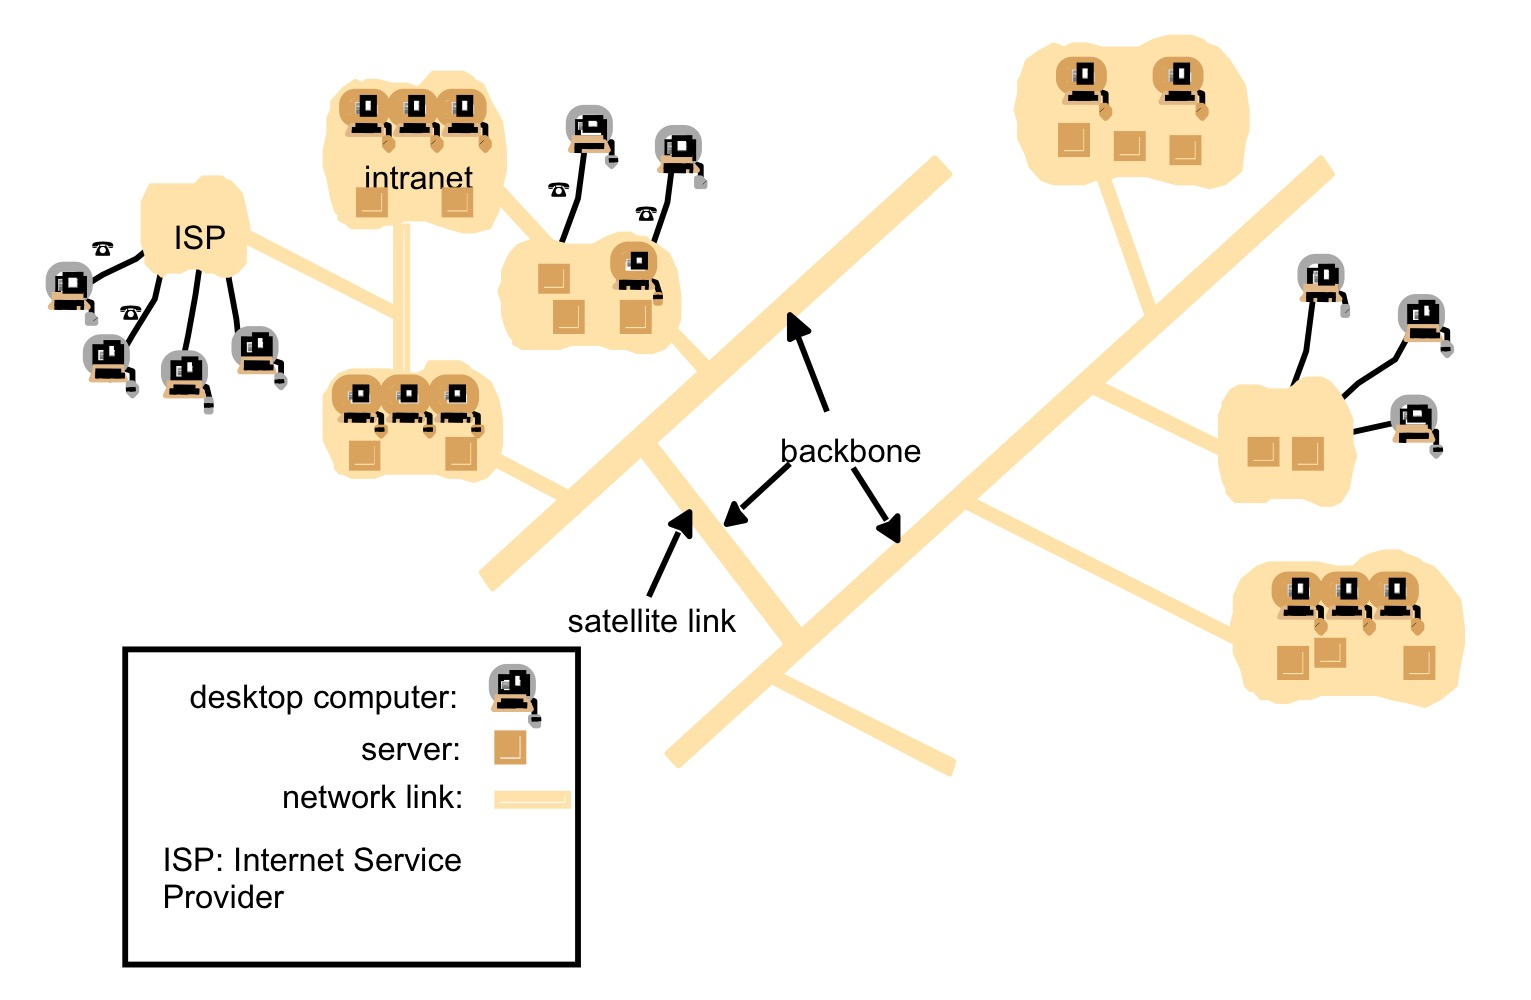
\includegraphics[width=.7\linewidth]{images/introduction/InternetAsDistributedSystem.jpeg}
    \caption{Internet as Distributed System}
\end{figure}

\section{Goals}
\begin{itemize}
    \item \textbf{Economy:} since data can be shared is not necessary to replicate it
    \item \textbf{Software:} the implementation follows particular standards
    \item \textbf{Flexibility:} gives a clear interface to use the system
    \item \textbf{Availability:} the system detects faults and applies recovery operations
    \item \textbf{Performance:} optimal performance in term of:
        \begin{itemize}
            \item Response time
            \item Throughput
            \item Parallelism
            \item Bottleneck reduction
        \end{itemize}
    \item \textbf{Locality and control distribution, security and efficiency} 
    \item \textbf{Transparency}
\end{itemize}

\section{Computer System vs Distributed System}
\begin{itemize}
    \item A \textit{Computer System} is characterised by \textit{single hardware}, system software and application software for data or control
    \item A \textbf{Distributed System} is composed of \textbf{distributed hardware} that can have or not \textbf{distribute software / application} to manage data and control
        \begin{itemize}
            \item \textbf{Distributed hardware:} system composed of \textit{more than two computer systems}, interconnected by a communication network and each \textit{computer is independent} from the others but can \textit{interact with them}
        \end{itemize}
\end{itemize}

\subsection{Control}
Control is essential to manage physical or logical resource on the system, it can be:
\begin{itemize}
    \item \textbf{Centralized:} there is a unique responsible entity
    \item \textbf{Distributed:} computer system on the net cooperate to reach the solution
    \item \textbf{Hierarchical:} system is more scalable since all the functions are subdivided in different modules
\end{itemize}

\section{Open Problems}
\begin{itemize}
    \item \textbf{Data Sharing:} understands how and what resources must be shared and it provides a \textit{system to retrieve them} efficiently
    \item \textbf{Heterogeneity:} enables users to access services and run applications over a heterogeneous collection of computers and networks
    \item \textbf{Concurrency}: several clients could attempt to access a \textit{shared resources} at the same time. The process that administrates shared resources could take one client request at a time.
    \item \textbf{Openness:} \textit{the system is not completely defined}, but it is possible to extend it, for instance \textit{including a new machine}. Open distributed system can be constructed from heterogeneous hardware and software, possibly from different vendors
    \item \textbf{Middleware:} is an intermediate layer that provides an unique public interface
    \item \textbf{Mobility:} it refers to \textit{program code} that can be \textit{transferred} from one computer to another and run at the destination
    \item \textbf{Security:} it is necessary to develop a secure system that \textit{does not allow unauthorized} users to read / write data:
        \begin{itemize}
            \item \textit{Confidentiality:} protection against revelation to unauthorized individuals
            \item \textit{Integrity:} protection against alteration or corruption
            \item \textit{Availability:} protection against interference
        \end{itemize}
    \item \textbf{Scalability:} if it remains stable even if there is a significant increase in the number of resources and users
    \item \textbf{Quality of Services (QoS):} reliability, security and performance of the entire system
    \item \textbf{Fault management:} faults need o be \textit{transparent to the user}. One of the most common recovery algorithm is \textbf{"checkpoint and rollback"} in which we go back the last checkpoint to recover the last consistent state
    \item \textbf{Transparency:} system is perceived as a \textit{set} instead of a \textit{collection of independent components}. Moreover we can analyse different type of transparency:
        \begin{itemize}
            \item \textit{Access:} enables local and remote resources using identical operations
            \item \textit{Location:} enables resources to be accessed without knowledge of their location
            \item \textit{Concurrency:} enables several processes to operate concurrently using shared resources without interface between them
            \item \textit{Replication:} enables multiple instances of resources to be used ti increase reliability and performance without knowledge of the replicas
            \item \textit{Failure:} enable the hiding of faults. Allowing users and application programs to complete their tasks despite the failure of hardware or software components
            \item \textit{Mobility:} allows the movement of resources and clients within a system without affecting the operation of users or programs
            \item \textit{Performance:} allows the system to be reconfigured to improve performance as loads vary
            \item \textit{Scaling:} the system and applications can expand in scale without change to the system structure
        \end{itemize}
\end{itemize}

\section{WWW as Example}
World Wide Web can be seen as a large distributed system based on Internet and its characteristics are:
\begin{itemize}
    \item \textbf{Open System:} it can be \textit{extended and implemented} in new ways without distributing its existing functionality 
    \item \textbf{Client-server architecture}
    \item \textbf{Transparency:}  using DNS it reaches the \textit{location transparency}. With the usage of symbolic server names it is not necessary for the client to know the exact physical address IP of the server
\end{itemize}